\documentclass[preview]{standalone}
\renewcommand\familydefault{\sfdefault}
\usepackage{amsmath,amssymb}
\usepackage{tikz}
\usetikzlibrary{shapes,arrows.meta,decorations.markings}

\begin{document}
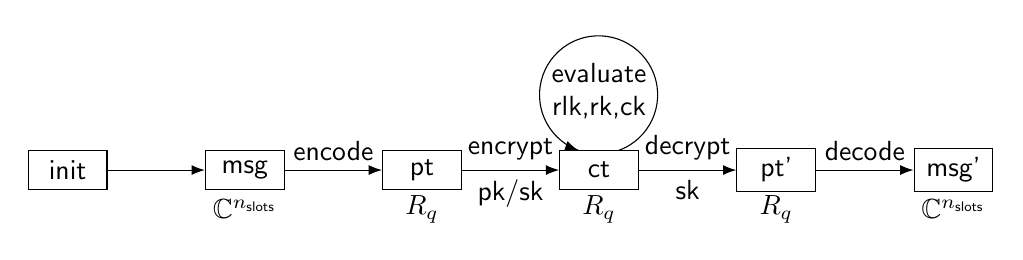
\begin{tikzpicture}
  \tikzstyle{place}     =[circle,draw=blue!50,fill=blue!20,thick]
  \tikzstyle{transition}=[rectangle,draw=black!50,fill=black!20,thick]
  \tikzstyle{rect}      =[draw, rectangle, minimum width=1cm, minimum height=0.5cm, align=center]
  \node[rect](r0) at (-2.25,0) {init};
  \node[rect](r1) at ( 0,0) {msg};
  \node[rect](r2) at ( 2.25,0) {pt};
  \node[rect](r3) at ( 4.5 ,0) {ct};
  \node[rect](r4) at ( 6.75,0) {pt'};
  \node[rect](r5) at ( 9   ,0) {msg'};
  \node at (0   ,-0.5){$\mathbb{C}^{n_{\text{slots}}}$};
  \node at (2.25,-0.5){$R_q$};
  \node at (4.5 ,-0.5){$R_q$};
  \node at (6.75,-0.5){$R_q$};
  \node at (9   ,-0.5){$\mathbb{C}^{n_{\text{slots}}}$};
  \draw[-Latex] (r0.east) -- (r1.west);
  \draw[-Latex] (r1.east) -- (r2.west) node[midway, above]{encode};
  \draw[-Latex] (r2.east) -- (r3.west) node[midway, above]{encrypt} node[midway, below]{pk/sk};
  \draw[-Latex] (r3.east) -- (r4.west) node[midway, above]{decrypt} node[midway, below]{sk};
  \draw[-Latex] (r4.east) -- (r5.west) node[midway, above]{decode};
  \draw[postaction={decorate,decoration={markings,mark=at position 1 with {\arrow{Latex}}}}] (4.75,0.25) arc (-70:250:0.75);
  \node[align=center, text width=1.5cm] at (4.5,1) {evaluate\\rlk,rk,ck};
\end{tikzpicture}
\end{document}
